\section{Experimental Evaluation}

We have evaluated our sensor planning solutions for gas emission monitoring in large environments, and conducted experiments in a indoor complex environment of size 000 $\times$ 00 m. Our robotic platform, as shown in Fig. 1, is Husky-200 which is running Robot Operating System (ROS), and equipped with an RMLD remote methane sensor and a pan-tilt unit. It is also equipped with the other sensors to navigation through the environment. In all the experiments, gas sampling was performed using sensing configurations of parameters $\phi = 270$\dg, and $r = 15$ m. 

One of the experiments is shown in Fig. \ref{fig:exp}. ... 

\begin{figure}[h!]
	\centering
	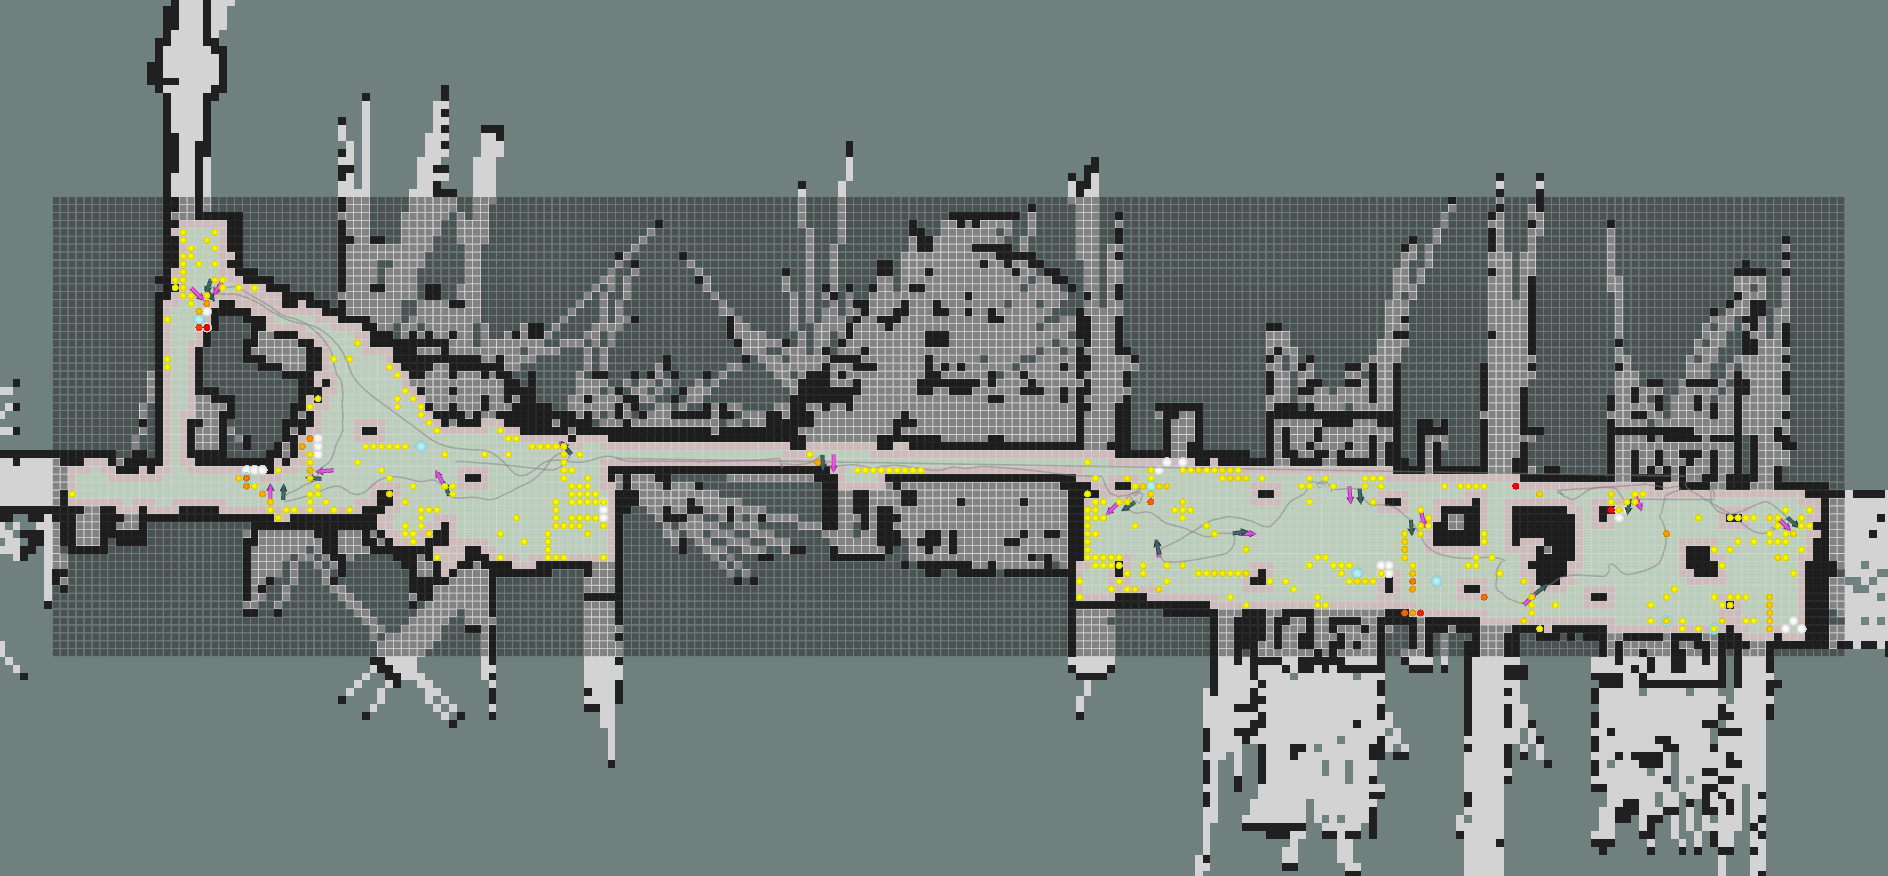
\includegraphics[trim={35 160 25 150}, clip,width=1\linewidth,angle=0]{fig/5-10-1se.png}
	%\vspace{1em}	
	\caption{...}
	\label{fig:exp}
\end{figure}


%\begin{figure}[H]
%	\centering
%	\includegraphics[trim={25 160 25 150}, clip,width=1.1\linewidth,angle=0]{fig/\x.png}
%	%\vspace{1em}
%	%\label{fig:\x}
%	\caption{Reconstruction.}
%\end{figure}


%\foreach \x in {01,02,03,04,05,06,07,08,09,10,11,12,13,14,15,16,17,18}
%{	
%	\begin{figure}[H]
%		\centering
%		\includegraphics[trim={25 160 25 150}, clip,width=1.1\linewidth,angle=0]{fig/\x.png}
%		%\vspace{1em}
%		%\label{fig:\x}
%		\caption{Reconstruction \#\x.}		
%	\end{figure}
%}
